\chapter{Data Visualization}

La Data Visualization è definita come la rappresentazione visiva dei dati attraverso l'utilizzo di modelli e grafici. Essa è posta al livello più alto dello stack infrastrutturale perché è il mezzo attraverso il quale viene mostrato il risultato dell'intera catena di processi operanti sui dati. Il motivo per cui è necessario utilizzare la visualizzazione nasce dall'incapacità del cervello umano di estrarre le informazioni utili presenti nei dati a partire dalla visione degli stessi nella loro forma grezza; tale informazione può però essere presentata in una forma interpretabile attraverso l'utilizzo di uno o più grafici. È quindi necessario che i grafici costruiti siano il più chiari, intuitivi e informativi possibile. Nello stack implementato è stato utilizzato come software di visualizzazione Tableau e, nel capitolo, è illustrata la sua struttura e quelli che sono i suoi punti di forza.

\section{Introduzione a Tableau}

Tableau è un software per la produzione di visualizzazioni dedicate alla Business Intelligence. Secondo Gartner \cite{gartner_tableau}, Tableau offre un'esplorazione visuale intuitiva e altamente interattiva attraverso l'accesso, la manipolazione e l'analisi dei dati senza la necessità di scrivere codice, posizionandosi tra i primi 3 prodotti leader nel suo settore. Tra gli elementi che distinguono Tableau c'è la semplicità e l'intuitività nell'utilizzo del software, la gestione dei data source e alcune caratteristiche innovative come le table calculation e la possibilità di fare analisi dati direttamente sui grafici. L'applicazione utilizzata On Premise si compone di due elementi:
\begin{itemize}
    \item \textbf{Tableau Desktop}: Permette la creazione di worksheet, dashboard e story collegate ad una o più sorgente di dati.
    \item \textbf{Tableau Server}: È utilizzato per pubblicare i grafici creati con Tableau Desktop al fine di renderli disponibili online.
\end{itemize}
\section{Tableau Desktop}

Tableau utilizza una struttura basata su workbook e sheet in stile Microsoft Excel: un workbook è composto da un insieme di sheet che possono assumere il ruolo di worksheet, dashboard, o story. Un worksheet contiene un singolo grafico con i relativi filtri e la sua legenda mentre un insieme di worksheet formano una dashboard. Una sequenza di dashboard crea invece una story che è solitamente la vista condivisa e mostrata all'utente finale. Alla base di ogni workbook c'è una o più sorgenti con le quali Tableau si connette per ricevere i dati da utilizzare.

\subsection{Data Source}

Il primo passo nella creazione di un workbook è quello di collegare Tableau ad un data source \cite{data_tableau}. Tableau Desktop supporta la connessione, attraverso connettori dedicati, a svariate fonti dati che possono essere raggruppati in due categorie: File e Server. Per quanto riguarda i File, sono supportati tutti i principali file di testo e relative formattazioni come JSON, CSV o TSV, i file in formato PDF, i fogli di calcolo Excel e i file Extract di Tableau. Per le connessioni ai Server, sono disponibili connettori ottimizzati per database relazionali come Microsoft SQL Server, database non relazioni come MongoDB e per sorgenti dati in cloud come Google Analytics, Amazon Redshift, e Salesforce. Nel caso in cui non sia presente l'interfaccia desiderata, è sempre possibile creare il proprio driver attraverso l'utilizzo di un ODBC\footnote{ODBC: Open DataBase Connectivity è una Application Programming Interface (API) per l'accesso ad un DBMS}. L'interazione con qualunque data source è gestito in maniera automatica da Tableau con \textbf{VizQL} (Visual Query Language). VizQL si occupa di tradurre le azioni di drag-and-drop eseguite in query adatte alla sorgente dati utilizzata al fine di rappresentare i risultati in maniera visuale attraverso dimensioni, forme e colori nei grafici. Una volta collegato Tableau al data source è possibile scegliere due tipologie di connessioni: Live e Extract.

\paragraph{Live}

La connessione live prevede l'interrogazione da parte di Tableau direttamente al data source; per questo motivo l'efficienza e le performance sono strettamente dipendenti da quelle del database utilizzato. In questo modo è però possibile aggiornare le visualizzazioni ogni qualvolta i dati vengono modificati ottenendo un grafico che si aggiorna teoricamente in tempo reale.

\paragraph{Extract}

La connessione extract prevede l'esecuzione della query sul data source e il salvataggio dei dati in un file Tableau Data Extract che verrà utilizzato per le successive interrogazioni. L'Extract può essere visto quindi come uno snapshot del database e, per questo motivo, le modifiche apportate non saranno visibili fino ad un aggiornamento del file. La creazione di un extract può richiedere diverso tempo ma il suo utilizzo si rileva estremamente efficiente data la struttura colonnare ottimizzata per il motore di esecuzione di Tableau.

\subsection{Creazione di una vista}

Ad ogni campo della tabella caricata dal sorgente viene associato un ruolo: dimensione o misura. Una dimensione rappresenta un'informazione categorica discreta come, ad esempio, una stringa o una data; una misura è invece un'informazione numerica e quantitativa potenzialmente aggregabile. È comunque possibile cambiare liberamente il ruolo di ogni campo a seconda dell'esigenza, così come passare da valori discreti a continui. Tramite drag-and-drop si spostano dimensioni e misure su ascisse e ordinate e Tableau automaticamente interpreta le variabili per costruire il grafico più significativo. Affinché le viste siano facilmente interpretabili, Tableau consente solamente la costruzione di grafici bi-dimensionali; la facoltà di aggiungere dimensioni, e quindi informazione, è data dall'utilizzo dei colori, della size e delle forme. I grafici che possono essere usati sono svariati, a partire da quelli classici come le torte, gli istogrammi, i bar chart, fino ad arrivare a grafici complessi dati dalla combinazione, tramite la tecnica del dual axis, di grafici elementari. Una nota di riguardo si ha per i grafici basati sulle mappe geografiche; Tableau infatti gestisce e interpreta, grazie ad alcuni dataset interni, i campi come gli stati, le regioni, le città, gli aeroporti e i codici postali come dimensioni geografiche utilizzabili sulla mappa. Una volta completato il grafico è possibile inserire diverse tipologie di filtri; scelta la dimensione o la misura da filtrare è necessario scegliere il tipo di filtro da applicare, ad esempio a singola o multipla scelta per le dimensioni mentre a valore esatto o a range per le misure. Esiste una sezione dedicata per le date in cui è possibile usare filtri assoluti o relativi rispetto ad una data e scegliere la granularità da utilizzare, a partire dall'anno fino ad arrivare al singolo secondo. Dimensioni e misure possono essere combinate insieme per creare un nuovo campo, definito calculated field, utilizzando funzioni matematiche e logiche. L'ultimo elemento di base utilizzabile è il parametro che consente di creare un campo che cambia in maniera dinamica con l'interazione dell'utente.

\subsubsection{Table calculation}

La Table Calculation è una delle caratteristiche innovative presenti in Tableau \cite{tableCalculation_tableau}. A differenza di tutte le altre operazioni che sono eseguite a livello di data source, esse insistono sui dati aggregati che compongono la vista; il calcolo è quindi eseguito utilizzando la cache di Tableau, come mostrato in Figura \ref{fig:TableCalculation}.

\begin{figure}[ht]
    \begin{center}
        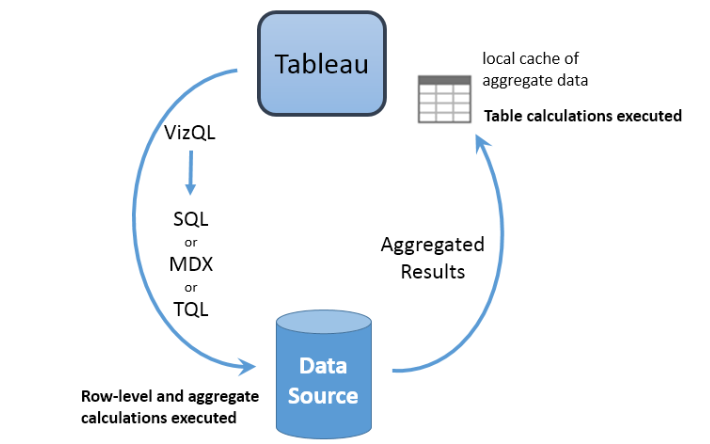
\includegraphics[width=0.8\linewidth]{Figures/TableCalculation.png}
    \end{center}
    \caption{Flusso di esecuzione di una table calculation \protect\cite{tableauFlow_image}.}
    \label{fig:TableCalculation}
\end{figure}

Il software mette a disposizione una lunga serie di operazioni utilizzabili ma lascia anche la possibilità all'utente di scrivere la propria table calculation. Una volta scelta la misura da indagare tra le varie possibilità proposte ci sono:

\begin{itemize}
    \item Calcolare il totale corrente (running total).
    \item Calcolare le evoluzioni temporali sia in valore assoluto sia in percentuale.
    \item Calcolare la media mobile o la percentile.
    \item Classificare e/o ordinare secondo una funzione di ranking/sorting.
\end{itemize}

\subsubsection{Analisi}

Una seconda caratteristica che rende Tableau particolarmente interessante è l'opportunità di eseguire analisi statistiche attraverso modelli matematici pre-caricati in Tableau o, in aggiunta, è anche possibile integrare algoritmi scritti in linguaggio R o in MatLab \cite{analisi_tableau}. Le analisi che possono essere eseguite usando i modelli pre-esistenti sono principalmente di 3 tipi:

\begin{itemize}
    \item Linee di trend: Ogni linea di tendenza aggiunta al grafico rappresenta un modello statistico di regressione lineare; in particolare Tableau costruisce la curva migliore usando 4 diversi tipi di funzioni: lineare, logaritmica, esponenziale e polinomiale.
    \item Previsioni (forecasting): Nel caso in cui sia presente una serie temporale, è possibile effettuare una previsione su un certo campo quantitativo utilizzando il metodo "exponential smoothing". Tale modello calcola i valori futuri sulla base di una funzione esponenziale che assegna i pesi al valore corrente e alla media dei valori passati; Tableau ricerca anche eventuali pattern ciclici in base al tipo di aggregazione eseguita, come ad esempio quella mensile o semestrale.
    \item Clustering: I dati vengono raggruppati in cluster sulla base delle variabili scelte. L'algoritmo utilizzato da Tableau è il K-Means in cui il valore di K è assegnato in maniera automatica; è comunque possibile modificare manualmente il numero di cluster da utilizzare.
\end{itemize}

\section{Tableau Server}

Tableau Server è un'applicazione server in grado di ospitare data source e workbook condivisi attraverso Tableau Desktop. Grazie al server, coloro che ne hanno diritto, sono in grado di vedere, interagire, scaricare, condividere e modificare un worksheet senza avere la necessità di installare Tableau Desktop sul proprio device; infatti è sufficiente utilizzare un browser web che supporti HTML5 o l'app mobile di Tableau. Inoltre, attraverso la condivisione del data source già autenticato, un utente è in grado di creare nuovi worksheet senza dover installare e mantenere i driver necessari ai connettori sul proprio computer. L'utilizzo di Tableau Server è però vincolato al possesso di un account.

\subsection{Embedded Tableau}

Tableau Server offre la possibilità di incorporare un worksheet in un sito internet o in un'applicazione web. In particolare, per quanto riguarda la web app, si utilizzano le Tableau JavaScript API che mettono a disposizione diverse funzioni e la possibilità di:

\begin{itemize}
    \item Visualizzare ed interagire con la vista condivisa.
    \item Caricare e ridimensionare la vista in maniera dinamica.
    \item Scaricare la vista come PDF o immagine.
\end{itemize}

Al primo tentativo di caricamento della vista è richiesto l'inserimento delle proprie credenziali in una finestra di login di Tableau Server. Tuttavia se vogliamo che ogni utente della web app sia in grado di visionare i grafici, nonostante non sia in possesso di un account Tableau, è possibile autenticare non il singolo utente ma il server che ospita l'applicazione. Per fare ciò è necessario seguire una procedura, denominata "Trusted Authentication", che sarà implementata nel caso di studio. 